\documentclass[11pt,letterpaper]{article}
\usepackage[margin=0.6in]{geometry}
\usepackage{amsmath,amssymb}
\usepackage{tikz}
\usetikzlibrary{arrows.meta,positioning}
\usepackage{xcolor}
\usepackage{fontawesome5}
\usepackage{tcolorbox}
\usepackage{multicol}
\usepackage{enumitem}
\usepackage{hyperref}

\definecolor{primaryblue}{RGB}{41, 98, 255}
\definecolor{accentgreen}{RGB}{0, 150, 136}
\definecolor{warnorange}{RGB}{255, 152, 0}
\definecolor{lightgray}{RGB}{245, 245, 245}

\tcbset{
    conceptbox/.style={colback=primaryblue!5, colframe=primaryblue, boxrule=1pt, arc=3pt, left=5pt, right=5pt, top=5pt, bottom=5pt},
    formulabox/.style={colback=lightgray, colframe=gray!50, boxrule=0.5pt, arc=2pt, left=5pt, right=5pt, top=3pt, bottom=3pt},
    warningbox/.style={colback=warnorange!10, colframe=warnorange, boxrule=1pt, arc=3pt, left=5pt, right=5pt, top=5pt, bottom=5pt},
    appbox/.style={colback=accentgreen!5, colframe=accentgreen, boxrule=1pt, arc=3pt, left=5pt, right=5pt, top=5pt, bottom=5pt}
}

\pagestyle{empty}
\setlength{\parindent}{0pt}
\setlist[itemize]{leftmargin=*, itemsep=1pt, topsep=2pt}

\begin{document}

\begin{center}
{\LARGE\bfseries\color{primaryblue} Chapter 8: Numerical Methods}\\[3pt]
{\large Floating Point, Stability, and Debugging}
\end{center}
\vspace{-5pt}
\hrule height 2pt
\vspace{8pt}

\begin{multicols}{2}

\begin{tcolorbox}[conceptbox, title={\faLightbulb\ Key Concepts}]
\begin{itemize}
    \item \textbf{Floating Point}: Finite precision $\Rightarrow$ rounding errors
    \item \textbf{Machine Epsilon}: Smallest distinguishable difference
    \item \textbf{Overflow/Underflow}: Numbers too large/small
    \item \textbf{Catastrophic Cancellation}: Subtraction of similar values
    \item \textbf{Numerical Stability}: Algorithms that control error growth
\end{itemize}
\end{tcolorbox}

\begin{tcolorbox}[formulabox, title={\faCalculator\ Core Formulas}]
\textbf{Log-Sum-Exp Trick:}
\[ \log \sum_i e^{x_i} = m + \log \sum_i e^{x_i - m} \]
where $m = \max_i x_i$

\textbf{Stable Softmax:}
\[ \text{softmax}(x)_i = \frac{e^{x_i - \max(x)}}{\sum_j e^{x_j - \max(x)}} \]

\textbf{Gradient Check:}
\[ \frac{\partial f}{\partial x} \approx \frac{f(x+\epsilon) - f(x-\epsilon)}{2\epsilon} \]
\end{tcolorbox}

\columnbreak

\begin{center}
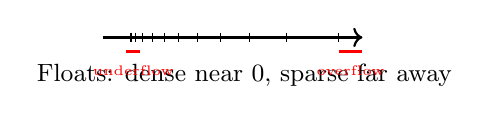
\begin{tikzpicture}[scale=0.6]
    % Number line showing float distribution
    \draw[->,thick] (-0.5,0) -- (5,0);

    % Dense near zero
    \foreach \x in {0.1,0.2,0.35,0.55,0.8,1.1,1.5,2,2.6,3.4,4.5} {
        \draw (\x,0.1) -- (\x,-0.1);
    }

    \node at (2.5,-0.8) {\small Floats: dense near 0, sparse far away};

    % Underflow region
    \draw[red,very thick] (0,-0.3) -- (0.3,-0.3);
    \node[red] at (0.15,-0.7) {\tiny underflow};

    % Overflow region
    \draw[red,very thick] (4.5,-0.3) -- (5,-0.3);
    \node[red] at (4.75,-0.7) {\tiny overflow};
\end{tikzpicture}
\end{center}

\vspace{5pt}

\begin{tcolorbox}[appbox, title={\faRobot\ ML Applications}]
\begin{itemize}
    \item \textbf{Mixed Precision Training}: FP16 forward, FP32 gradients
    \item \textbf{Loss Scaling}: Prevent gradient underflow
    \item \textbf{Gradient Clipping}: Prevent exploding gradients
    \item \textbf{LayerNorm/BatchNorm}: Numerical stability
\end{itemize}
\end{tcolorbox}

\begin{tcolorbox}[warningbox, title={\faExclamationTriangle\ Debugging Checklist}]
\begin{itemize}
    \item \textbf{NaN?} Check for $\log(0)$, $0/0$, $\sqrt{\text{negative}}$
    \item \textbf{Inf?} Check for overflow, division by tiny number
    \item \textbf{Loss explodes?} Learning rate too high, gradient explosion
    \item \textbf{Loss stuck?} Vanishing gradients, dead ReLUs
    \item Always use \texttt{log\_softmax} not \texttt{log(softmax)}
\end{itemize}
\end{tcolorbox}

\end{multicols}

\vspace{5pt}
\hrule
\vspace{5pt}

\begin{center}
\faGithub\ \textbf{Notebook}: \url{https://github.com/vijaygwu/math-powers-ai/blob/main/notebooks/ch08_numerical_methods.ipynb}
\end{center}

\end{document}
